\documentclass{article}
\usepackage[utf8]{inputenc}
\usepackage[T1]{fontenc}

\usepackage{graphicx}
\usepackage{subcaption}

\usepackage{ifxetex}
\ifxetex
  \usepackage{fontspec}
\else
  \usepackage[T1]{fontenc}
  \usepackage[utf8]{inputenc}
  \usepackage{lmodern}
\fi

\title{Reporte de Actividad 8}
\author{Roberto Benard Orci}
\date{12/03/2018}

\begin{document}
\maketitle

\section{Introducción}

En esta actividad estudiaremos el oscilador de Van Der Pol, el cual es un oscilador con amortiguamiento no lineal. El oscilador cumple con la siguiente ecuación:

 \begin{equation}
 \frac{d^2p}{dt^2} -\mu (1-x^2)\frac{dp}{dt} + x = 0
 \end{equation}
 
En donde \textit{x} representa la posición, \textit{t} el timepo, y $\mu$ es un parametro escalar que representa el amortiguamiento o la no linealidad. 

\subsection{Antecedentes}

Van Der Pol estudiaba circuitos cuando encontró ciertas oscilaciones estables, que llamó oscilaciones de relajación, ahora conocidas como ciclos límite. Este fue uno de los primeros descubrimientos experimentales de la teoría del caos.

Hoy en día, esta ecuación tiene distintas aplicaciones en varias áreas de la ciencia.


\section{Modelo de Van de Pol}

Algunos de los diferentes modelos para los que se usa la ecuación de Van Der Pol serian los siguientes: 

\vspace{0.3cm}

\noindent - Oscilaciones de cuerdas vocales.

\noindent - Fallas geológicas.

\noindent - Potencial de acción, impulsos eléctricos, en la membrana celular.

\vspace{0.3cm}

Todos estos pueden ser modelados por la ecuación de Van Der Pol ya que son sistemas caóticos no lineales. Un sistema caótico es un sistema dinámico que que es muy sensible a sus condiciones iniciales. 

\vspace{0.3cm}

Aplicando la transformación de Liénard uno puede probar que el sistema tiene un ciclo limite, este es el \textit{Teorema de Liénard}. De esta manera el oscilador de Van Der Pol se convierte en una forma de dos dimensiones. 

 \begin{equation}
 \frac{dx}{dt} = y
 \end{equation}
 
  \begin{equation}
 \frac{dy}{dt} =\mu (1-x^2)y - x = 0
 \end{equation}
 
 Algo interesante es que en el caso donde no hay fuerza, cuando $\mu$\textit{=0}, la ecuación se vuelve:

 \begin{equation}
 \frac{d^2x}{dt^2} + x = 0
 \end{equation}
 
 Esta es la forma de un oscilador armónico simple.
 
 \subsection{Hamiltoniano y oscilador forzado}
 
 El \textit{Hamiltoniano} describe la evolución de un sistema, para el oscilador de Van Der Pol, este quedaria de la siguiente manera:
 
 \begin{equation}
 \frac{d^2x}{dt^2} -\mu (1-x^2)\frac{dx}{dt} + x = 0
 \end{equation}
 
  \begin{equation}
 \frac{d^2y}{dt^2} -\mu (1-x^2)\frac{dy}{dt} + x = 0
 \end{equation}
 
 \vspace{0.3cm}
 
 En el caso en que el sistema modelado por la ecuación de Van Der Pol sea alterado constantemente por un factor externo, se le puede agregar un conjunto de variables a la ecuación para que esta represente un sistema forzado. La ecuación queda de la siguiente manera:
 
  \begin{equation}
 \frac{d^2p}{dt^2} -\mu (1-x^2)\frac{dp}{dt} + x -ASin(\omega t) = 0
 \end{equation}
 
 Donde \textit{A} representa la amplitud, y $\omega$ la velocidad angular.

\subsection{Caos determinista}

Me gusto el concepto de caos determinista, como un sistema caótico, como lo es casi todo en la naturaleza, puede ser modelado con un serie de ecuaciones diferenciales. En el articulo muestran un ejemplo de un circuito eléctrico y como al conectar un un teléfono se oían diferentes sonidos, antes se consideraba un fenómeno extraño, hoy en dia, se sabe que era caos determinista.  

\vspace{1cm}

\section{Exploración de las soluciones del modelo en el Espacio Fase}

Las siguientes gráficas muestran las ecuaciones de Van Der Pol usando una constante $\mu$ \textit{= 3.00} y diferentes condiciones iniciales.



\begin{figure}[h!]
  \centering
  \begin{subfigure}[b]{0.45\linewidth}
    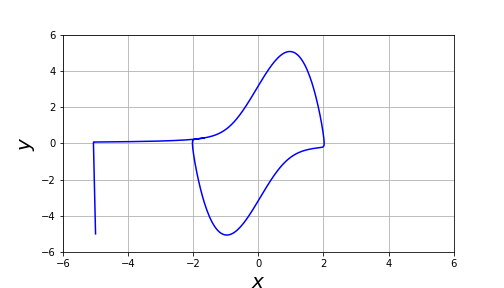
\includegraphics[width=\linewidth]{EspacioFase1.png}
     \caption{}
  \end{subfigure}
  \begin{subfigure}[b]{0.45\linewidth}
    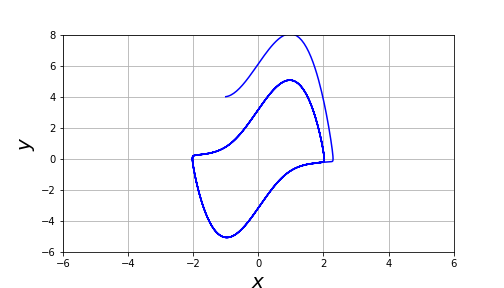
\includegraphics[width=\linewidth]{EspacioFase3.png}
    \caption{}
  \end{subfigure}
  \begin{subfigure}[b]{0.45\linewidth}
    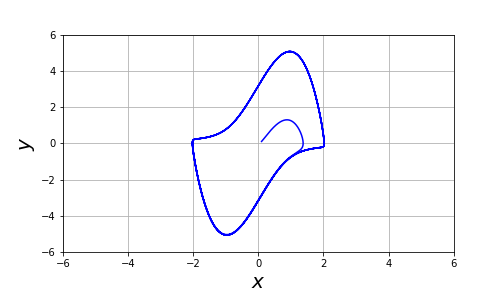
\includegraphics[width=\linewidth]{EspacioFase4.png}
    \caption{}
  \end{subfigure}
  \begin{subfigure}[b]{0.45\linewidth}
    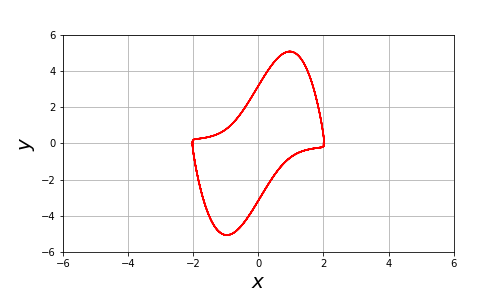
\includegraphics[width=\linewidth]{EspacioFase.png}
    \caption{}
  \end{subfigure}
\end{figure}

\vspace{0.3cm}

Como se puede ver, sin importar las condiciones iniciales del sistema, este eventualmente terminara igual que en la gráfica \textit{(d)}, su movimiento tendera al ciclo limite, tal y como se comprobó con el \textit{Teorema de Liénard}. 
 
\section{Resultados}

En esta actividad replicamos las gráficas  de wikipedia sofre el oscilador de Van Der PoL, estos fueron los resultados:

\begin{center}
	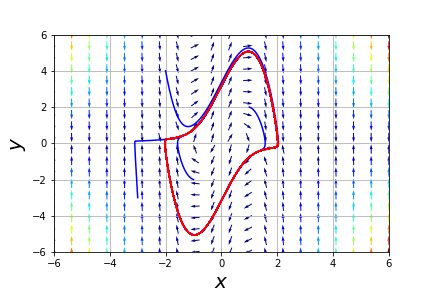
\includegraphics[width=10cm]{PrimeraFig.png}
    
\end{center}
\vspace{0.3cm}

Esta gráfica es muy parecida a las que se mostraron anteriormente, solo que es una combinación de diferentes condiciones iniciales. Ahora es mas facial observar a lo que se refería cuando se menciono el movimiento de la gráfica, este seguirá a los vectores de la gráfica hasta tomar la forma del ciclo limite. 

\begin{center}
	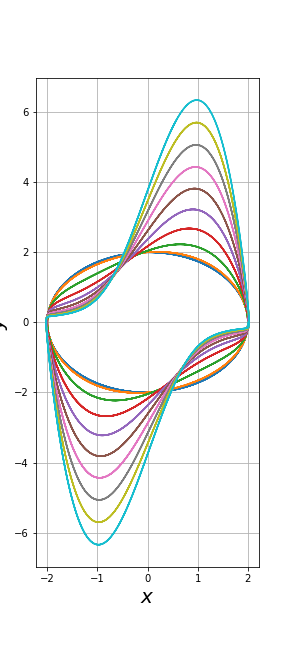
\includegraphics[width=6cm]{SegundaFig.png}
    
\end{center}
\vspace{0.3cm}

Esta gráfica muestra la evolución del ciclo limite, con valores empezando con valores pequeños de $\mu$, formando los óvalos en el centro, aumentando el tamaño de las curvas.

\vspace{2cm}

\begin{center}
	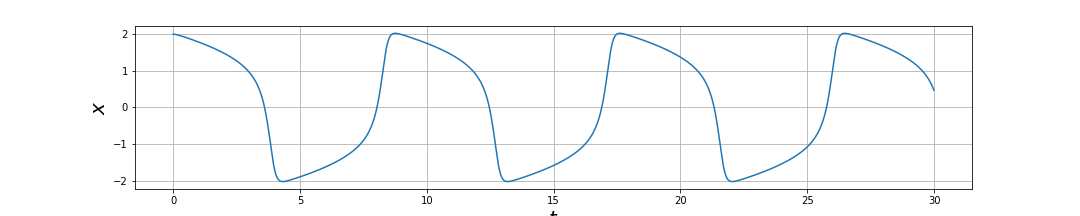
\includegraphics[width=13cm]{TerceraFig.png}
    
\end{center}
\vspace{0.3cm}

En esta otra gráfica se muestra el movimiento normal de las oscilaciones.

\begin{center}
	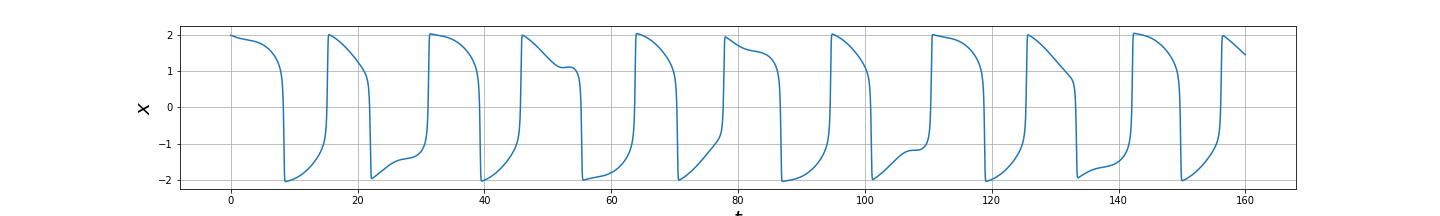
\includegraphics[width=13cm]{CuartaFig.png}
    
\end{center}
\vspace{0.3cm}

Aquí se puede observar un ejemplo de una oscilación forzada. En comparación con la gráfica anterior, esta tiene pequeñas alteraciones en sus oscilaciones.
 
 
\section{Conclusión}

La naturaleza esta gobernada por sistemas caóticos, los cuales pueden ser modelados por ecuaciones diferenciales para mejorar su comprensión, para encontrar un ciclo limite, y observar a los diferentes movimientos a los que puede tender un sistema.


\section{Bilbiografía}

\begin{verbatim}
Van der Pol oscillator. (2018, April 10). Retrieved April 11, 2018,
from https://en.wikipedia.org/wiki/Van_der_Pol_oscillator 
\end{verbatim}
%https://en.wikipedia.org/wiki/Van_der_Pol_oscillator

\begin{verbatim}
Matplotlib: Lotka volterra tutorial¶. (n.d.). Retrieved April 11, 2018, 
from http://scipy-cookbook.readthedocs.io/items/LoktaVolterraTutorial.html 
\end{verbatim}
%http://scipy-cookbook.readthedocs.io/items/LoktaVolterraTutorial.html

\begin{verbatim}
Kanamaru, T. (n.d.). Van der Pol oscillator. Retrieved April 11, 2018, 
from http://www.scholarpedia.org/article/Van_der_Pol_oscillator 
\end{verbatim}
%http://www.scholarpedia.org/article/Van_der_Pol_oscillator

\section{Apéndice}


    1.- Este ejercicio pareciera similar al desarrollado en las actividades 6 y 7. ¿Qué aprendiste nuevo?
    
    \vspace{0.3cm}
	El uso de vectores en el grid que apunten hacia la dirección de movimiento del sistema.
    \vspace{0.3cm}
    
\noindent 2.- ¿Qué fue lo que más te llamó la atención del oscilador de Van der Pol? 
    
    \vspace{0.3cm}
	Los diferentes usos que se le dan, en la biológica y en la física. 
    \vspace{0.3cm}
    
\noindent    3.- Has escuchado ya hablar de caos. ¿Por qué sería importante estudiar este oscilador?
    
    \vspace{0.3cm}
	Por que son sistemas que dependen mucho de sus condiciones iniciales, al igual que muchos problemas de la vida diaria.
    \vspace{0.3cm}
    
\noindent    4.- ¿Qué mejorarías en esta actividad?
    
    \vspace{0.3cm}
	Diferentes modelos en los que se puedan usar los vectores como grid para visualizar el movimiento del sistema.
    \vspace{0.3cm}
    
\noindent    5.- ¿Algún comentario adicional antes de dejar de trabajar en Jupyter con Python?
    
    \vspace{0.3cm}
	Me gusto el uso de Python en Jupyter.
    \vspace{0.3cm}
    
\noindent    6.- Cerramos la parte de trabajo con Python ¿Que te ha parecido?
    
    \vspace{0.3cm}
	En general me gusto mucho, el tener que importar distintas bibliotecas dependiendo de lo que vayas a hacer me hace sentir que estoy personalizando mas el código.
    \vspace{0.3cm}


\end{document}